\section{Marco teórico específico}

Java RMI, introducido en el JDK 1.1, es una implementación de RPC específica para el ecosistema Java. A diferencia de ONC RPC o gRPC, su IDL es el propio lenguaje Java: una interfaz que extiende \texttt{java.rmi.Remote} describe el contrato del servicio remoto. La especificación oficial de Oracle describe tres componentes principales: el \textbf{stub}, representante local del objeto remoto en el cliente, que empaqueta los argumentos y abre la conexión con la JVM remota; el \textbf{skeleton} (contraparte en el servidor, generado dinámicamente desde Java~2 mediante \texttt{java.lang.reflect.Proxy}, por lo que ya no requiere generación explícita); y el \textbf{registro RMI} (\texttt{rmiregistry}), servicio de nombres en el que el servidor publica el objeto remoto (\texttt{Naming.rebind}) y desde el que el cliente lo localiza (\texttt{Naming.lookup}). El protocolo de transporte por defecto es JRMP (Java Remote Method Protocol) sobre TCP.

\textit{Nota de alcance:} esta implementación integra desde el inicio dos elementos que el instructivo plantea como reto de extensión (bitácora persistente y RMI sobre TLS), en vez de construir primero una versión mínima y refactorizarla después. Las secciones de este capítulo señalan explícitamente qué corresponde al ejercicio base y qué corresponde a la extensión, y el reto de extensión (Sección~\ref{sec:p2-reto}) documenta la evidencia específica de esas dos capacidades.

\section{Entorno de trabajo}

Esta práctica requiere dos procesos JVM independientes —servidor y cliente— comunicándose por red. Siguiendo el entorno común descrito en el marco teórico general, se utilizaron dos contenedores Docker (\texttt{rmi-servidor} y \texttt{rmi-cliente}) sobre una misma imagen \texttt{fedora:36} con JDK~17, conectados por una red de Docker dedicada (\texttt{pcta2-net}) que simula dos nodos en una red local, exponiendo el puerto 1099/TCP del \texttt{rmiregistry} dentro de esa red.

\begin{lstlisting}[language=bash]
$ docker network create pcta2-net
$ docker run -d --name rmi-servidor --network pcta2-net \
    --cap-add=NET_ADMIN --cap-add=NET_RAW pcta2-rmi sleep infinity
$ docker run -d --name rmi-cliente --network pcta2-net pcta2-rmi sleep infinity
\end{lstlisting}

\begin{figure}[H]
\centering
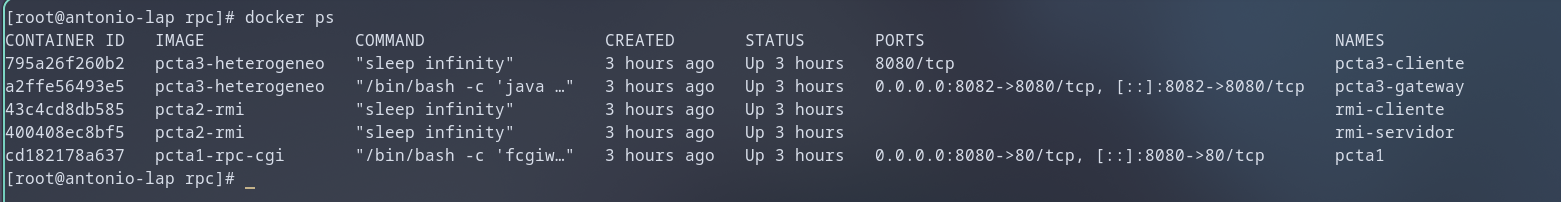
\includegraphics[width=\linewidth]{../src/ss/3.1.png}
\caption{Contenedores \texttt{rmi-servidor} y \texttt{rmi-cliente} en ejecución sobre la red \texttt{pcta2-net}.}
\label{fig:p2-docker-ps}
\end{figure}

En la Figura~\ref{fig:p2-docker-ps} destacan dos aspectos. Primero, los contenedores \texttt{rmi-servidor} y \texttt{rmi-cliente} no publican ningún puerto hacia el anfitrión (columna \texttt{PORTS} vacía): a diferencia de la práctica 1, la comunicación ocurre íntegramente dentro de la red interna \texttt{pcta2-net}, donde Docker provee resolución de nombres automática —el cliente localiza al servidor por el nombre \texttt{rmi-servidor}, no por una IP. Segundo, ambos corren la misma imagen \texttt{pcta2-rmi} con \texttt{sleep infinity} como proceso principal: los procesos JVM se lanzan después con \texttt{docker exec}, lo que permite tratar cada contenedor como un ``nodo'' genérico en el que se arranca el rol deseado, tal como se haría con dos máquinas físicas.

\section{Estructura del proyecto}

\begin{lstlisting}[language=bash]
src/mx/ipn/esimecu/rpc/
  Calculadora.java       # interfaz remota
  CalculadoraImpl.java   # implementación (con bitácora)
  BitacoraRemota.java    # interfaz del segundo objeto remoto (reto)
  BitacoraRemotaImpl.java# implementación de la bitácora (reto)
  ServidorRMI.java       # arranque del servidor
  ClienteRMI.java        # cliente que invoca
\end{lstlisting}

\section{Interfaz remota --- \texttt{Calculadora.java}}

\begin{lstlisting}[language=Java]
package mx.ipn.esimecu.rpc;

import java.rmi.Remote;
import java.rmi.RemoteException;

public interface Calculadora extends Remote {
    double sumar(double a, double b)        throws RemoteException;
    double restar(double a, double b)       throws RemoteException;
    double multiplicar(double a, double b)  throws RemoteException;
    double dividir(double a, double b)      throws RemoteException;
    String quienSoy()                       throws RemoteException;
}
\end{lstlisting}

\section{Implementación --- \texttt{CalculadoraImpl.java}}

Cada operación aritmética (ejercicio base) delega adicionalmente en el objeto remoto \texttt{BitacoraRemota} (extensión) para registrar la invocación:

\begin{lstlisting}[language=Java]
public class CalculadoraImpl extends UnicastRemoteObject implements Calculadora {
    private static final long serialVersionUID = 1L;
    private final BitacoraRemota bitacora;

    protected CalculadoraImpl(BitacoraRemota bitacora,
            RMIClientSocketFactory csf, RMIServerSocketFactory ssf) throws RemoteException {
        super(0, csf, ssf);
        this.bitacora = bitacora;
    }

    @Override public double sumar(double a, double b) throws RemoteException {
        double r = a + b; log("sumar", a, b, r); return r;
    }
    // restar, multiplicar análogos ...

    @Override
    public double dividir(double a, double b) throws RemoteException {
        if (b == 0.0) {
            bitacora.registrar("dividir(" + a + ", " + b + ") -> ERROR división entre cero");
            throw new RemoteException("División entre cero");
        }
        double r = a / b; log("dividir", a, b, r); return r;
    }
}
\end{lstlisting}

\section{Servidor --- \texttt{ServidorRMI.java}}

El servidor publica dos objetos remotos: la calculadora y la bitácora, ambos exportados mediante \texttt{SslRMIClientSocketFactory}/\texttt{SslRMIServerSocketFactory} (extensión: RMI sobre TLS):

\begin{lstlisting}[language=Java]
public class ServidorRMI {
    public static void main(String[] args) throws Exception {
        SslRMIClientSocketFactory csf = new SslRMIClientSocketFactory();
        SslRMIServerSocketFactory ssf = new SslRMIServerSocketFactory();

        LocateRegistry.createRegistry(1099);

        BitacoraRemota bitacora = new BitacoraRemotaImpl(Path.of("/tmp/bitacora.log"), csf, ssf);
        Naming.rebind("rmi://localhost:1099/BitacoraIPN", bitacora);

        Calculadora servicio = new CalculadoraImpl(bitacora, csf, ssf);
        Naming.rebind("rmi://localhost:1099/CalculadoraIPN", servicio);
    }
}
\end{lstlisting}

\section{Cliente --- \texttt{ClienteRMI.java}}

\begin{lstlisting}[language=Java]
public class ClienteRMI {
    public static void main(String[] args) throws Exception {
        String host = args.length > 0 ? args[0] : "localhost";
        Calculadora c = (Calculadora) Naming.lookup("rmi://" + host + ":1099/CalculadoraIPN");
        BitacoraRemota b = (BitacoraRemota) Naming.lookup("rmi://" + host + ":1099/BitacoraIPN");

        System.out.println("Conectado a " + c.quienSoy());
        System.out.println("3 + 4  = " + c.sumar(3, 4));
        System.out.println("10 - 6 = " + c.restar(10, 6));
        System.out.println("7 * 8  = " + c.multiplicar(7, 8));
        try { System.out.println("5 / 0  = " + c.dividir(5, 0)); }
        catch (Exception e) { System.out.println("Error remoto controlado: " + e.getMessage()); }

        b.consultar().forEach(System.out::println);
    }
}
\end{lstlisting}

\section{Compilación y ejecución}

\begin{lstlisting}[language=bash]
# --- Servidor (contenedor rmi-servidor) ---
$ javac -encoding UTF-8 src/mx/ipn/esimecu/rpc/*.java
$ java $RMI_TLS_OPTS -Djava.rmi.server.hostname=rmi-servidor \
    mx.ipn.esimecu.rpc.ServidorRMI
Servidor RMI (TLS) listo en rmi://localhost:1099/CalculadoraIPN
Bitácora remota publicada en rmi://localhost:1099/BitacoraIPN
\end{lstlisting}
\begin{figure}[H]
\centering
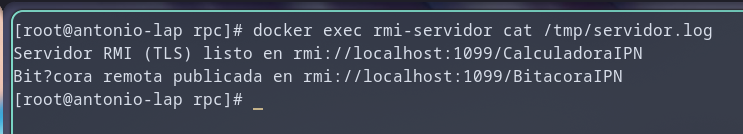
\includegraphics[width=0.85\linewidth]{../src/ss/3.2.png}
\caption{Bitácora de arranque del servidor RMI: registro creado y ambos objetos remotos publicados.}
\label{fig:p2-servidor}
\end{figure}

Los dos mensajes de la Figura~\ref{fig:p2-servidor} confirman la secuencia de publicación descrita en el marco teórico específico: \texttt{LocateRegistry.createRegistry(1099)} arranca el \texttt{rmiregistry} embebido en el propio proceso, y a continuación dos llamadas a \texttt{Naming.rebind} asocian los nombres lógicos \texttt{CalculadoraIPN} y \texttt{BitacoraIPN} con sus objetos exportados. Desde ese momento el servicio de nombres puede responder consultas \texttt{Naming.lookup} de cualquier cliente de la red. Nótese que el registro cumple el mismo papel que la tabla de \emph{locations} de nginx en la práctica 1: es el directorio que traduce un nombre público a un procedimiento concreto, pieza del \emph{runtime} de RPC encargada del descubrimiento del servicio.

\begin{lstlisting}[language=bash]
# --- Cliente (contenedor rmi-cliente), invocando al servidor por su nombre en la red Docker ---
$ java $RMI_TLS_OPTS mx.ipn.esimecu.rpc.ClienteRMI rmi-servidor
Conectado a Calculadora remota en 400408ec8bf5/172.18.0.2
3 + 4  = 7.0
10 - 6 = 4.0
7 * 8  = 56.0
Error remoto controlado: RemoteException occurred in server thread; nested exception is:
	java.rmi.RemoteException: División entre cero

--- Historial (BitacoraRemota) ---
2026-07-20T00:49:47.241 | sumar(3.0, 4.0) = 7.0
2026-07-20T00:49:47.255 | restar(10.0, 6.0) = 4.0
2026-07-20T00:49:47.258 | multiplicar(7.0, 8.0) = 56.0
2026-07-20T00:49:47.268 | dividir(5.0, 0.0) -> ERROR división entre cero
\end{lstlisting}
\begin{figure}[H]
\centering
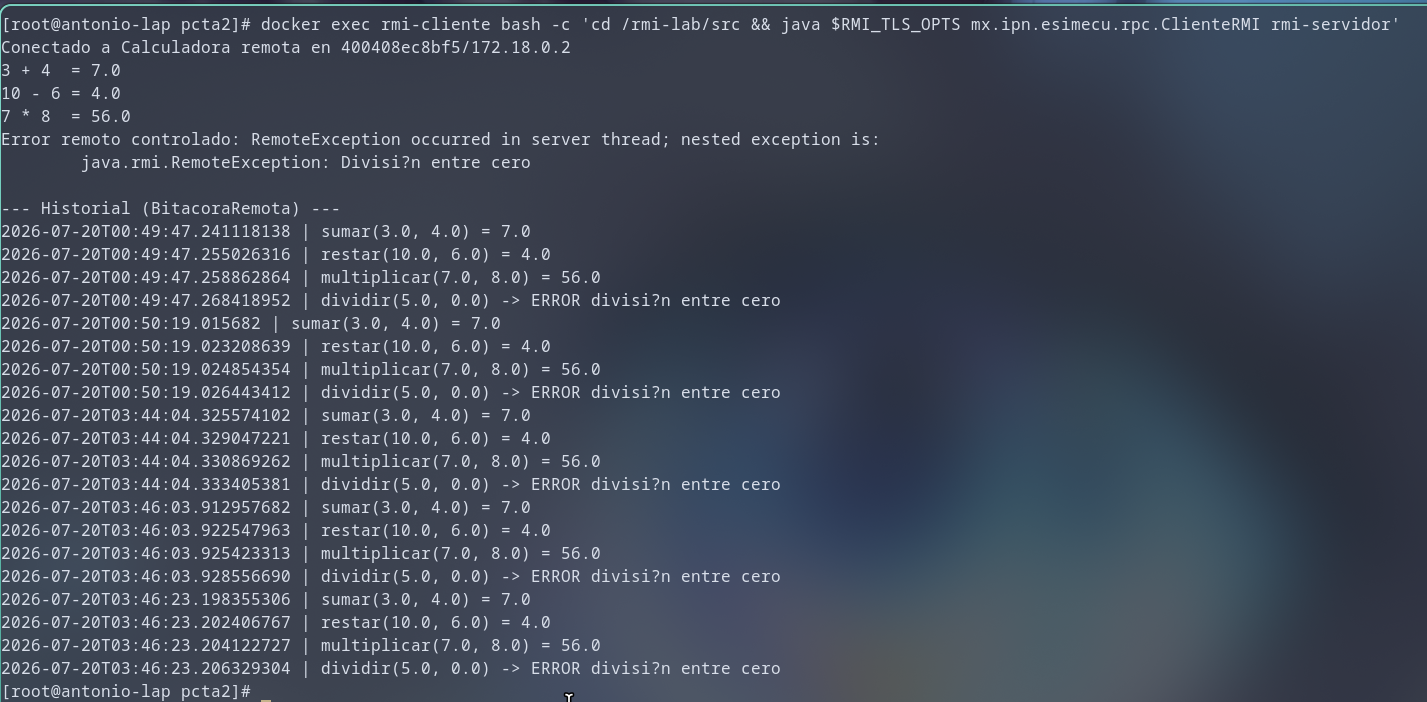
\includegraphics[width=\linewidth]{../src/ss/3.4.png}
\caption{Ejecución del cliente RMI: invocaciones remotas, excepción controlada e historial consultado a \texttt{BitacoraRemota}.}
\label{fig:p2-cliente}
\end{figure}

La Figura~\ref{fig:p2-cliente} condensa varios principios del modelo. La línea \texttt{Conectado a Calculadora remota en 400408ec8bf5/172.18.0.2} prueba que la respuesta proviene de la otra JVM (el \emph{hostname} y la IP son los del contenedor servidor, no los del cliente). Las tres operaciones aritméticas se invocan con sintaxis de llamada local (\texttt{c.sumar(3, 4)}) pese a ejecutarse en otro nodo: transparencia sintáctica lograda por el stub dinámico que \texttt{Naming.lookup} construyó. La división entre cero muestra el límite de la transparencia semántica: el error de negocio llega envuelto en una \texttt{RemoteException} —el mismo tipo que señalaría una caída de red— porque en RMI todo fallo remoto, sea de la lógica o del transporte, atraviesa el mismo canal de excepciones declarado en la interfaz. Finalmente, el historial impreso al pie es el resultado de invocar al \emph{segundo} objeto remoto (\texttt{BitacoraRemota}) y demuestra que el servidor conservó estado de ejecuciones anteriores: las entradas con marcas de tiempo distintas corresponden a corridas separadas del cliente.

Las invocaciones se realizaron entre dos contenedores distintos comunicados por red (\texttt{172.18.0.2} y \texttt{172.18.0.3}), reproduciendo la topología de dos nodos que pide el instructivo sin necesidad de dos máquinas físicas.

\section{Análisis de tráfico}

Se distinguieron dos tramos de comunicación con \texttt{tcpdump}: la resolución de nombres contra \texttt{rmiregistry} en el puerto 1099 (en texto plano, ya que el registro en sí no se exportó con \emph{sockets} SSL) y la invocación real de los métodos remotos en un puerto efímero negociado dinámicamente, protegido con TLS por las fábricas \texttt{SslRMIClientSocketFactory}/\texttt{SslRMIServerSocketFactory}. El siguiente fragmento hexadecimal, capturado en ese puerto efímero (\texttt{39519} en esta ejecución), muestra el registro de protocolo TLS \emph{Handshake} (\texttt{0x16}) seguido de la versión de registro TLS~1.0 por compatibilidad (\texttt{0x0301}) y la versión negociada TLS~1.2 dentro del \emph{ClientHello} (\texttt{0x0303}):

\begin{lstlisting}
172.18.0.3.33630 > 172.18.0.2.39519: Flags [P.], length 408
0x0000: 4500 01cc c862 4000 4006 18a0 ac12 0003
0x0010: ac12 0002 835e 9a5f ca03 fcfe 8c2c 7c2e
0x0020: 8018 003f 59e8 0000 0101 080a baa8 a60d
0x0030: 4fde 67bc 1603 0301 9301 0001 8f03 0396
0x0040: ccb4 12cc 91b1 533c 5611 5fff c133 d9d0
\end{lstlisting}

\begin{figure}[H]
\centering
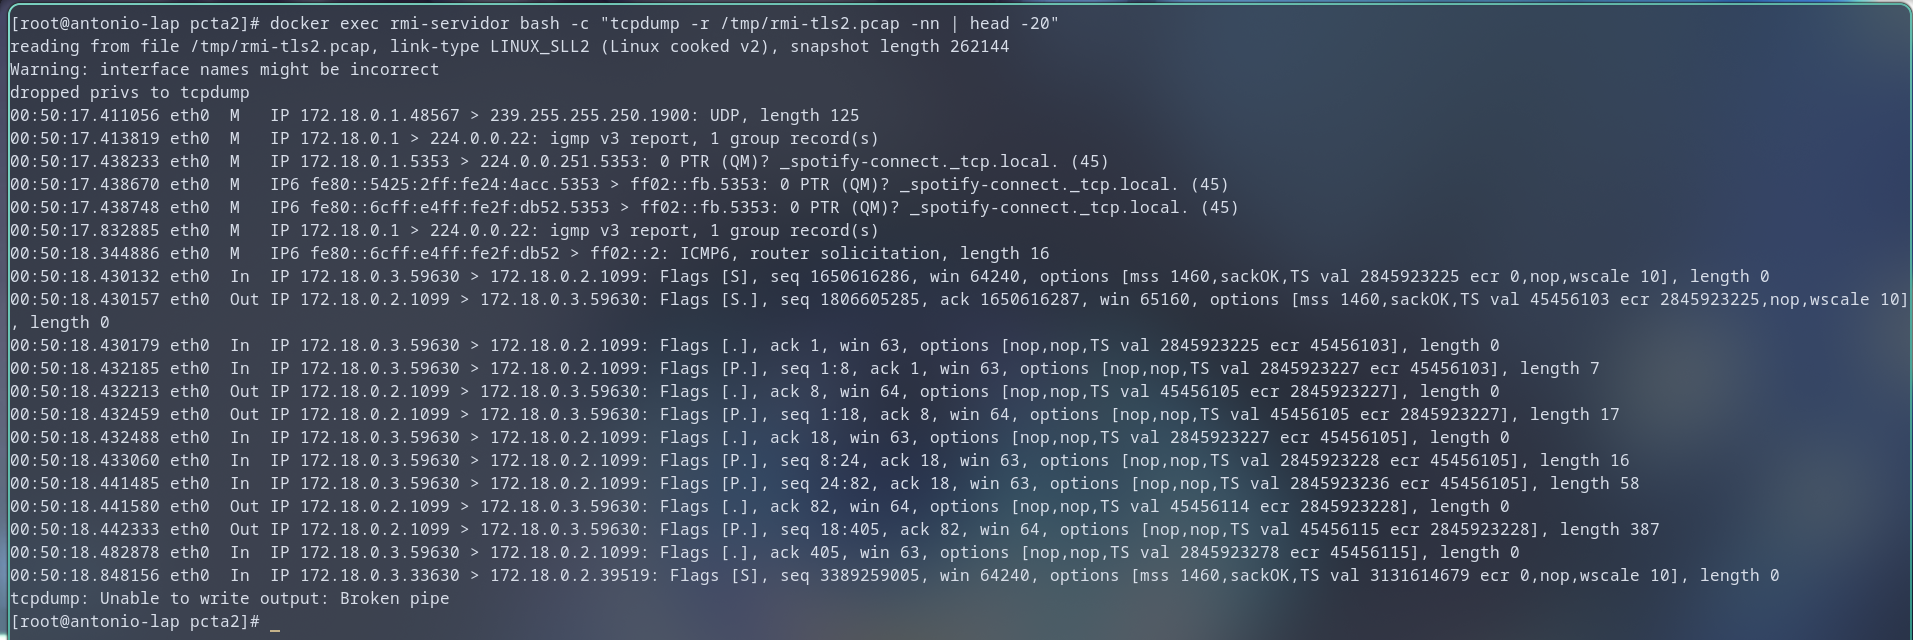
\includegraphics[width=\linewidth]{../src/ss/3.5.png}
\caption{Lectura de la captura con \texttt{tcpdump}: sesión JRMP contra el puerto 1099 y apertura de la conexión TLS en el puerto efímero 39519.}
\label{fig:p2-tcpdump}
\end{figure}

En la Figura~\ref{fig:p2-tcpdump} puede seguirse la anatomía de una invocación RMI a nivel de segmentos TCP. Primero, el saludo de tres vías (\emph{three-way handshake}: banderas \texttt{[S]}, \texttt{[S.]}, \texttt{[.]}) abre la conexión del cliente \texttt{172.18.0.3} hacia el puerto \texttt{1099} del servidor; los segmentos \texttt{[P.]} siguientes —de longitudes pequeñas: 7, 17, 16, 58 bytes— son el protocolo JRMP en claro negociando la consulta al registro, y el segmento de 387 bytes es la respuesta del \texttt{lookup}: contiene el stub serializado, que incluye la dirección y el puerto donde el objeto remoto real escucha. Con esa información, en la última línea el cliente abre una \emph{segunda} conexión hacia el puerto efímero \texttt{39519}: es el puerto que \texttt{UnicastRemoteObject} obtuvo al exportarse con la fábrica SSL, y todo lo que viaja por él va cifrado con TLS. La captura ilustra así el diseño de dos planos de RMI: un plano de descubrimiento (registro, en claro) y un plano de invocación (objeto, cifrado).

\section{Asociación con los cinco componentes RPC}

\begin{table}[H]
\centering
\caption{Asociación de la práctica 2 con la arquitectura clásica de RPC.}
\label{tab:componentes-rpc-p2}
\begin{tabularx}{\linewidth}{lX}
\toprule
\textbf{Componente RPC} & \textbf{Realización en Java RMI} \\
\midrule
Cliente & Clase \texttt{ClienteRMI} que invoca métodos como si la calculadora estuviese en memoria. \\
Stub del cliente & Proxy dinámico generado por la JVM al hacer \texttt{Naming.lookup}; serializa los argumentos primitivos con \texttt{ObjectOutputStream}. \\
RPC runtime & Transporte JRMP (sobre TLS para los objetos exportados) más \texttt{rmiregistry} para resolución de nombres y el \emph{thread pool} de \texttt{UnicastRemoteObject}. \\
Stub del servidor & Mecanismo interno de \texttt{UnicastRemoteObject} que recibe la invocación entrante y la dispacha por reflexión. \\
Servidor & Objetos \texttt{CalculadoraImpl} y \texttt{BitacoraRemotaImpl} que ejecutan la operación y retornan el resultado al stub. \\
\bottomrule
\end{tabularx}
\end{table}

\begin{figure}[H]
\centering
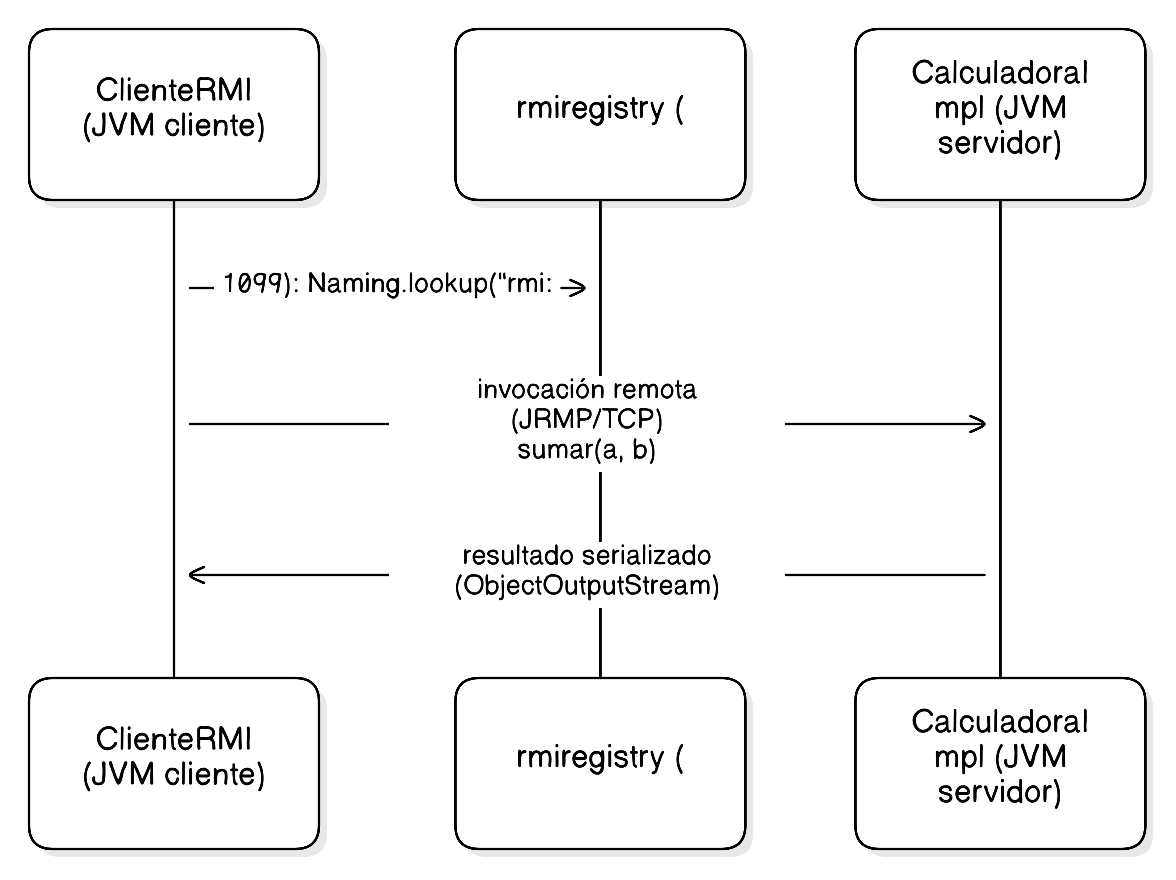
\includegraphics[width=0.85\linewidth]{../src/diagrams/practica2_secuencia.png}
\caption{Diagrama de secuencia de la invocación remota en Java RMI.}
\label{fig:p2-secuencia}
\end{figure}
